\section{Magnetische Induktion}

\vspace{1\baselineskip}

\fat{Der magnetische Fluss} durch eine Oberfläche $\vec{A}$ ist definiert durch
\begin{align*}
    \Phi_{\text{mag}} = \int_A \vec{B} \cdot d \vec{A}
\end{align*}

\vspace{1\baselineskip}

\begin{center} 
    \begin{minipage}{0.15\textwidth}
        \begin{center}
            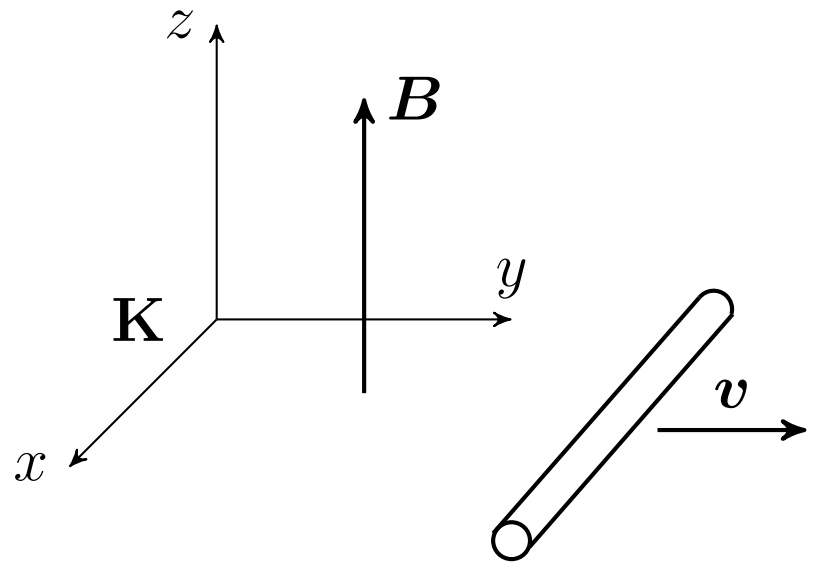
\includegraphics[width=\textwidth]{Figures/Induktion.png}
        \end{center}
    \end{minipage}\hspace{15pt}
    \begin{minipage}{0.3\textwidth}
        In der linken Darstellung gilt für den Stab mit Endpunkten $A$ und $B$:
        \begin{align*}
            U_{BA} = \int_A^B q (\vec{v} \times \vec{B}) \cdot d \vec{s}
        \end{align*}
    \end{minipage}
\end{center}

\vspace{1\baselineskip}

Die \fat{elektromotorische Kraft} ist dann gegeben als:
\begin{align*}
    \mathcal{E} = \oint_C \ (\vec{v} \times \vec{B}) \cdot d \vec{s} = \frac{U_{BA}}{q}
\end{align*}

\vspace{1\baselineskip}

\fat{Faraday'sches Gesetz}:
\begin{align*}
    \mathcal{E} = U_{\text{ind}} = - \frac{d \Phi_{\text{mag}}}{dt}
    = - \frac{d}{dt} \int_A \vec{B} \cdot d \vec{A}
\end{align*}

\vspace{1\baselineskip}

\fat{Das Lenz'sche Gesetz}

Die magnetisch induzierte elektromotorische Kraft erzeugt ihrerseits ein Magnetfeld, das der
Änderung des Flusses entgegenwirkt.

\vspace{1\baselineskip}

\begin{minipage}{0.2\textwidth}
    Die \fat{Leistung}, die eine externe Kraft $\vec{F}_{\text{ext}}$ aufbringen muss, um im
    Widerstand $R$ dissipierte Joul'sche Wärme zu ersetzen, ist gegeben durch
\end{minipage} \hspace{15pt}
\begin{minipage}{0.25\textwidth}
    \begin{center}
        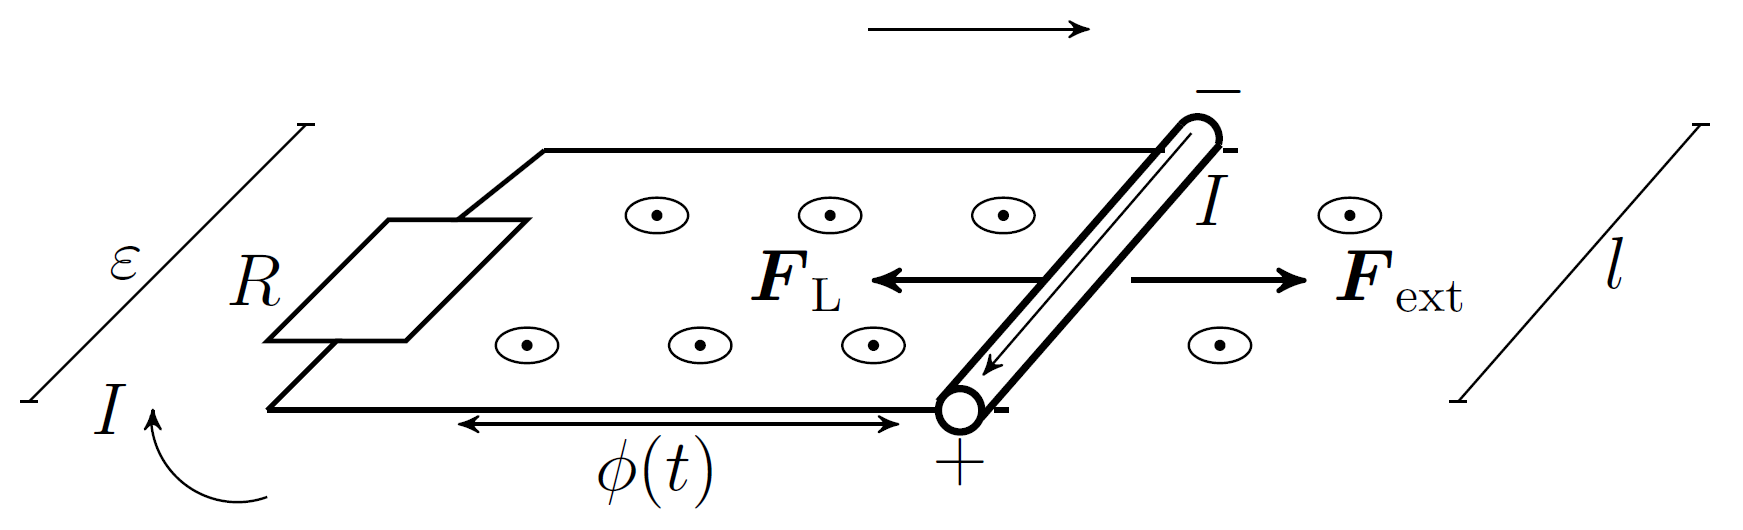
\includegraphics[width=\textwidth]{Figures/Lenz.png}
    \end{center}
\end{minipage}
\begin{align*}
    \vec{F}_{\text{ext}} \cdot \vec{v} = l I B v = \mathcal{E} I
    \quad \quad \quad \quad \quad \quad \text{ für diesen Aufbau}
\end{align*}

\vspace{1\baselineskip}

\fat{Selbstinduktion}

Der Strom durch eine Spule erzeugt ein Magnetfeld. Das Magnetfeld ist proportional zum Strom $I$.
Der magnetische Fluss ist:
\begin{align*}
    \Phi_{\text{mag}} = L I
\end{align*}
mit $L$ der \fat{Selbstinduktivität} der Spule. Die Spannung durch Selbstinduktion
ist nach dem Faraday'schen Gesetz:
\begin{align*}
    U_{\text{ind}} = -L \frac{dI}{dt}
\end{align*}

\vspace{1\baselineskip}

\fat{Gegenseitige Induktivität}
ist der Einfluss auf eine Spule, erzeugt durch eine andere Spule
\begin{align*}
    \Phi_{\text{mag},21} = M_{21} I_1
\end{align*}
mit $M_{21}$ der \fat{gegenseitigen Induktivität}. Es gilt: $M_{12} = M_{21}$

\vspace{1\baselineskip}

Das Magnetfeld einer langen Spule mit einer Querschnittsfläche $A$, Länge $l$ und
Anzahl Windungen $N$ ist gegeben als:
\begin{align*}
    B = \munull \frac{N}{l} I
\end{align*}
Dann folgt:
\begin{align*}
    &\Phi = \munull A \frac{N}{l} I N
    \quad \Longrightarrow \quad
    \mathcal{E}_{\text{ind}} = - \frac{d \Phi}{dt} = - \munull \frac{N^2}{l} A \frac{dI}{dt}
    \\
    &\Longrightarrow L = \munull \frac{A N^2}{l}
\end{align*}

\vspace{1\baselineskip}

\fat{Gespeicherte Energie}:
\begin{align*}
    U = \frac{1}{2} L I^2 = \frac{1}{2 \munull} \int_V B^2 dV
\end{align*}
